\documentclass[sigconf]{acmart}

\usepackage{graphicx}
\usepackage{hyperref}
\usepackage{todonotes}

\usepackage{endfloat}
\renewcommand{\efloatseparator}{\mbox{}} % no new page between figures

\usepackage{booktabs} % For formal tables

\settopmatter{printacmref=false} % Removes citation information below abstract
\renewcommand\footnotetextcopyrightpermission[1]{} % removes footnote with conference information in first column
\pagestyle{plain} % removes running headers

\newcommand{\TODO}[1]{\todo[inline]{#1}}

\begin{document}
\title{Hadoop and MongoDB in support of Big Data Applications and Analytics}


\author{Sushant Athaley}
\affiliation{%
  \institution{Indiana University}
}
\email{sathaley@iu.edu}

% The default list of authors is too long for headers}
\renewcommand{\shortauthors}{G. v. Laszewski}


\begin{abstract}
Big data processing is beyond capability of traditional tool. It requires specialized tools like Hadoop and MongoDB. We will explore Haddop and MongoDB technically as a tool and how they provide support/help in big data analysis.
TBD
\end{abstract}

\keywords{i523, hid302, big data, Hadoop, MongoDB}


\maketitle


\section{Introduction}

Describe about big data, hadoop and mongodb. Describe what this paper will do.
Papers organization.

\section{Big Data}
Big Data is defined in lot many different ways but one of the interesting ways it has been defined is in terms of three V's which are Volume, Velocity, and Variety. Big data is generated in great \emph{volume} typically in the gigabyte or more which makes data processing difficult. Data \emph{velocity} has been increased due to the real-time data streaming from various applications like social media or different type of sensors recording data continuously. Big data comes in \emph{variety} of format like structured or unstructured data. Data varies in various format like text, pictures, audio, videos, 3D, social media and so on. These big data characteristics pose challenges in terms of overall data lifecycle management. Some of the examples of big data usage are the recommendation service, predictive analytics, data analytics, pattern identification, and machine learning. Traditional systems are good for small or medium data processing but unable to provide support for the big data. Big data need specialized technologies and tools to handle its characteristics. The technologies which can solve big data problem should have capabilities like distributed computing system, massively parallel processing, NoSQL, and analytical database \cite[Ch.\ 1, p. 4]{AchariShiva2015HE}. Can Hadoop or MongoDB be those technologies who can provide that support?  

\section{Hadoop}
introduce hadoop, architecture, support to big data, real life examples
Apache foundation describes Hadoop as ``The Apache Hadoop software library is a framework that allows for the distributed processing of large data sets across clusters of computers using simple programming models. It is designed to scale up from single servers to thousands of machines, each offering local computation and storage. Rather than rely on hardware to deliver high-availability, the library itself is designed to detect and handle failures at the application layer, so delivering a highly-available service on top of a cluster of computers, each of which may be prone to failures'' \cite{www-hadoop}. In other words, Hadoop provides a framework to store data in the distributed manner and provides the capability to run data analysis in the distributed way.

``Currently Hadoop project includes following modules:
\begin{itemize}
\item {\bf Hadoop Common}: The common utilities that support the other Hadoop modules.
\item {\bf Hadoop Distributed File System (HDFS)}: A distributed file system that provides high-throughput access to application data.
\item {\bf Hadoop YARN}: A framework for job scheduling and cluster resource management.
\item {\bf Hadoop MapReduce}: A YARN-based system for parallel processing of large data sets'' \cite{www-hadoop}.
\end{itemize}

\subsection{Hadoop Common}

\subsection{Hadoop Distributed File System (HDFS)}
Hadoop Distributed File System (HDFS) is the default distributed file system provided by the Hadoop. HDFS serves as storage mechanism in the Hadoop framework. HDFC specifically designed to process large data set and run on low cost hardware. It is high fault tolerant which contains mechanism for quick fault detection and auto recovery. HDFS is designed to port across heterogeneous hardware and software platform. It does data computation on same node instead of moving data to the server which is faster as well as avoid network congestion. It provides scalability by adding or removing nodes in the HDFS cluster and can support hundreds of nodes in single cluster \cite{www-hdfs-arch}. Figure \ref{f:hdfs-arch} shows HDFS architecture.
\begin{figure}[!ht]
  \centering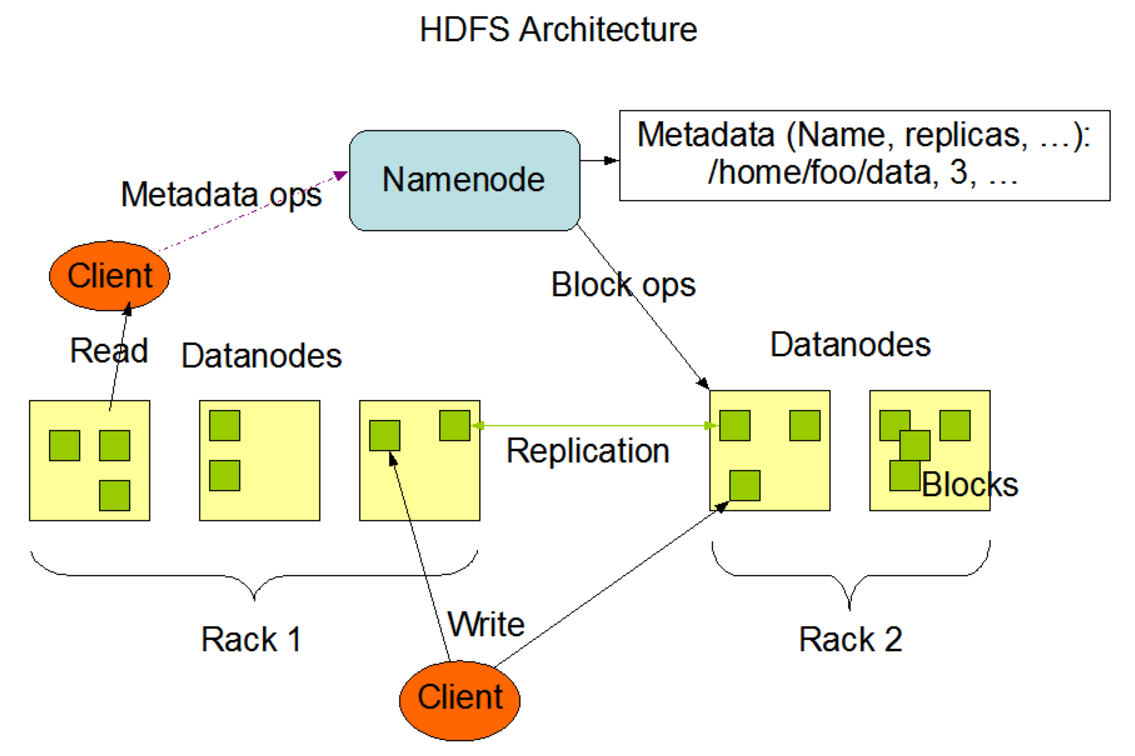
\includegraphics[width=\columnwidth]{images/hdfsArch.PNG}
  \caption{HDFS Architecture \cite{www-hdfs-arch}}\label{f:hdfs-arch}
\end{figure}

HDFS is based on master/slave architecture where NameNode is the master server and DataNodes are the slave nodes. There can be only one NameNode server which manages file system name space and all read write requests. NameNode doesn't store any data but contains all the meta-data about files and DataNodes. DataNode contains actual data and they can be multiple in numbers usually one per node. DataNodes are responsible for the create, delete, replicate of the datablocks on the node as per the instruction by the NameNode. It also sends heartbeat message to NameNode which helps in identifing the failure nodes. If heartbeat is not received by NameNode in specified interval then that DataNode is marked as dead and NameNode usage different DataNode.

\subsection{Hadoop YARN}

\subsection{Hadoop MapReduce}

\subsection{Big Data Support}

\section{MongoDB}


\section{Tables}

In case you need to create tables, you can do this with online tools
(if you do not mind sharing your data) such as
\url{https://www.tablesgenerator.com/} or other such tools (please
google for them). They even allow you to manage tables as CSV.

or generate them by hand while using the provided template in Table\ref{t:mytable}. Not ethat
the caption is before the tabular environment.

\begin{table}[htb]
\centering
\caption{My caption}
\label{t:mytabble}
\begin{tabular}{lll}
1 & 2 & 3 \\
\hline
4 & 5 & 6 \\
7 & 8 & 9
\end{tabular}
\end{table}

\section{Long example}

If you like to see a more elaborate example, please look at
report-long.tex. 

\section{Conclusion}

Put here an conclusion. Conlcusions and abstracts must not have any
citations in the section.


\begin{acks}

  The authors would like to thank Dr. Gregor von Laszewski for his
  support and suggestions to write this paper.

\end{acks}

\bibliographystyle{ACM-Reference-Format}
\bibliography{report} 

\appendix

We include an appendix with common issues that we see when students
submit papers. One particular important issue is not to use the
underscore in bibtex labels. Sharelatex allows this, but the
proceedings script we have does not allow this.

When you submit the paper you need to address each of the items in the
issues.tex file and verify that you have done them. Please do this
only at the end once you have finished writing the paper. To d this
cange TODO with DONE. However if you check something on with DONE, but
we find you actually have not executed it correcty, you will receive
point deductions. Thus it is important to do this correctly and not
just 5 minutes before the deadline. It is better to do a late
submission than doing the check in haste. 

\section{Issues}

\DONE{Example of done item: Once you fix an item, change TODO to DONE}

\subsection{Citation Issues and Plagiarism}

    \TODO{Put a space between the citation mark and the previous word}

\subsection{Details about the Figures and Tables}

    \TODO{In case you copied a figure from another paper, you must include a reference to the original in the caption}
    \TODO{Figures should be reasonably sized and often you just need to
  add columnwidth} e.g. \begin{verbatim}/includegraphics[width=\columnwidth]{images/myimage.pdf}\end{verbatim}

re


\end{document}
